
\documentclass[border=8pt, multi, tikz]{standalone} 
\usepackage{import}
\subimport{../../layers/}{init}
\usetikzlibrary{positioning}
\usetikzlibrary{3d} %for including external image 

\def\ConvColor{rgb:yellow,5;red,2.5;white,5}
\def\ConvReluColor{rgb:yellow,5;red,5;white,5}
\def\PoolColor{rgb:red,1;black,0.3}
\def\UnpoolColor{rgb:blue,2;green,1;black,0.3}
\def\FcColor{rgb:blue,5;red,2.5;white,5}
\def\FcReluColor{rgb:blue,5;red,5;white,4}

\def\FcFineColor{rgb:green,10;red,2.5;black,3}
\def\FcReluFineColor{rgb:green,10;red,8;black,3}

\def\SoftmaxColor{rgb:green,10;black,7}   
\def\SumColor{rgb:blue,5;green,15}

\newcommand{\copymidarrow}{\tikz \draw[-Stealth,line width=0.8mm,draw={rgb:blue,4;red,1;green,1;black,3}] (-0.3,0) -- ++(0.3,0);}

\begin{document}
\begin{tikzpicture}
\tikzstyle{connection}=[ultra thick,every node/.style={sloped,allow upside down},draw=\edgecolor,opacity=0.7]
\tikzstyle{copyconnection}=[ultra thick,every node/.style={sloped,allow upside down},draw={rgb:blue,4;red,1;green,1;black,3},opacity=0.7]

\pic[shift={(0,0,0)}] at (0,0,0) 
    {Box={
        name=input,
        caption=input,
        xlabel=3,
        ylabel=32,
        zlabel=96,
        fill=\ConvColor,
        height=32,
        width=3,
        depth=96
        }
    };

\node[canvas is zy plane at x=0] (temp) at (input-east) {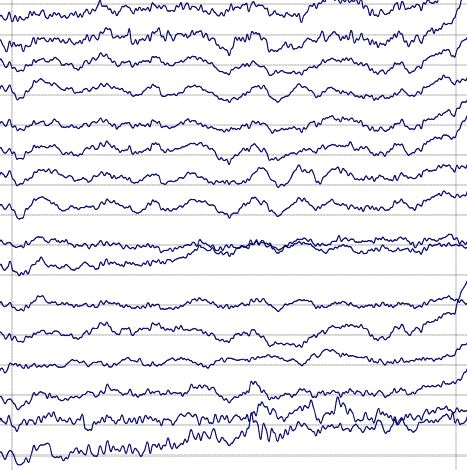
\includegraphics[width=18cm,height=6cm]{eeg.jpg}};

\pic[shift={(3,0,0)}] at (input-east) 
    {RightBandedBox={
        name=conv1,
        caption=conv1,
        xlabel=6,
        ylabel=28,
        zlabel=82,
        fill=\ConvColor,
        bandfill=\ConvReluColor,
        height=28,
        width=6,
        depth=82
        }
    };

\draw [connection]  (input-east)    -- node {\midarrow} (conv1-west);

\pic[shift={ (0,0,0) }] at (conv1-east) 
    {Box={
        name=pool1,
        caption=MaxPool,
        xlabel=6,
        ylabel=14,
        zlabel=40,    
        fill=\PoolColor,
        opacity=0.5,
        height=14,
        width=6,
        depth=40
        }
    };

\pic[shift={(3,0,0)}] at (pool1-east) 
    {RightBandedBox={
        name=conv2,
        caption=conv2,
        xlabel=8,
        ylabel=10,
        zlabel=26,
        fill=\ConvColor,
        bandfill=\ConvReluColor,
        height=10,
        width=8,
        depth=26
        }
    };

\draw [connection]  (pool1-east)    -- node {\midarrow} (conv2-west);

\pic[shift={ (0,0,0) }] at (conv2-east) 
    {Box={
        name=pool2,
        caption=MaxPool,
        xlabel=8,
        ylabel=5,
        zlabel=12,    
        fill=\PoolColor,
        opacity=0.5,
        height=5,
        width=8,
        depth=12
        }
    };

\pic[shift={(2,0,0)}] at (pool2-east) 
    {RightBandedBox={
        name=conv3,
        caption=conv3,
        xlabel=8,
        ylabel=5,
        zlabel=12,
        fill=\ConvColor,
        bandfill=\ConvReluColor,
        height=5,
        width=8,
        depth=12
        }
    };

\draw [connection]  (pool2-east)    -- node {\midarrow} (conv3-west);

\pic[shift={ (0,0,0) }] at (conv3-east) 
    {Box={
        name=pool31,
        caption=MaxPool,
        xlabel=8,
        ylabel=2,
        zlabel=4,    
        fill=\PoolColor,
        opacity=0.5,
        height=2,
        width=8,
        depth=4
        }
    };

\pic[shift={(0,15,0)}] at (0,0,0) 
    {Box={
        name=input,
        caption=input,
        xlabel=3,
        ylabel=32,
        zlabel=96,
        fill=\ConvColor,
        height=32,
        width=3,
        depth=96
        }
    };

\node[canvas is zy plane at x=0] (temp) at (input-east) {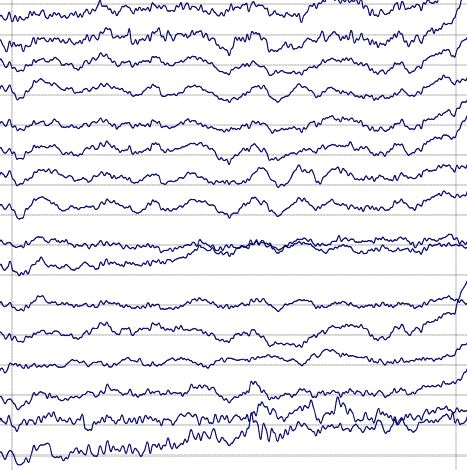
\includegraphics[width=18cm,height=6cm]{eeg.jpg}};

\pic[shift={(3,0,0)}] at (input-east) 
    {RightBandedBox={
        name=conv1,
        caption=conv1,
        xlabel=6,
        ylabel=28,
        zlabel=82,
        fill=\ConvColor,
        bandfill=\ConvReluColor,
        height=28,
        width=6,
        depth=82
        }
    };

\draw [connection]  (input-east)    -- node {\midarrow} (conv1-west);

\pic[shift={ (0,0,0) }] at (conv1-east) 
    {Box={
        name=pool1,
        caption=MaxPool,
        xlabel=6,
        ylabel=14,
        zlabel=40,    
        fill=\PoolColor,
        opacity=0.5,
        height=14,
        width=6,
        depth=40
        }
    };

\pic[shift={(3,0,0)}] at (pool1-east) 
    {RightBandedBox={
        name=conv2,
        caption=conv2,
        xlabel=8,
        ylabel=10,
        zlabel=26,
        fill=\ConvColor,
        bandfill=\ConvReluColor,
        height=10,
        width=8,
        depth=26
        }
    };

\draw [connection]  (pool1-east)    -- node {\midarrow} (conv2-west);

\pic[shift={ (0,0,0) }] at (conv2-east) 
    {Box={
        name=pool2,
        caption=MaxPool,
        xlabel=8,
        ylabel=5,
        zlabel=12,    
        fill=\PoolColor,
        opacity=0.5,
        height=5,
        width=8,
        depth=12
        }
    };

\pic[shift={(2,0,0)}] at (pool2-east) 
    {RightBandedBox={
        name=conv3,
        caption=conv3,
        xlabel=8,
        ylabel=5,
        zlabel=12,
        fill=\ConvColor,
        bandfill=\ConvReluColor,
        height=5,
        width=8,
        depth=12
        }
    };

\draw [connection]  (pool2-east)    -- node {\midarrow} (conv3-west);

\pic[shift={ (0,0,0) }] at (conv3-east) 
    {Box={
        name=pool32,
        caption=MaxPool,
        xlabel=8,
        ylabel=2,
        zlabel=4,    
        fill=\PoolColor,
        opacity=0.5,
        height=2,
        width=8,
        depth=4
        }
    };

\pic[shift={(0,30,0)}] at (0,0,0) 
    {Box={
        name=input,
        caption=input,
        xlabel=3,
        ylabel=32,
        zlabel=96,
        fill=\ConvColor,
        height=32,
        width=3,
        depth=96
        }
    };

\node[canvas is zy plane at x=0] (temp) at (input-east) {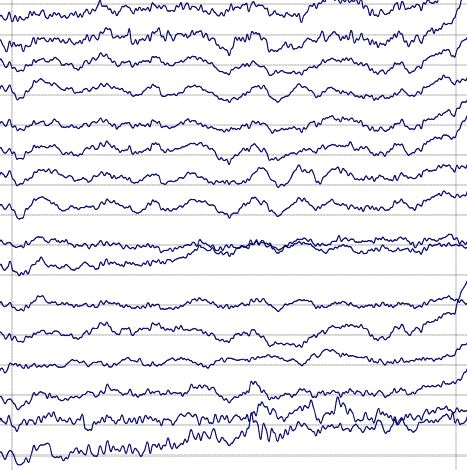
\includegraphics[width=18cm,height=6cm]{eeg.jpg}};

\pic[shift={(3,0,0)}] at (input-east) 
    {RightBandedBox={
        name=conv1,
        caption=conv1,
        xlabel=6,
        ylabel=28,
        zlabel=82,
        fill=\ConvColor,
        bandfill=\ConvReluColor,
        height=28,
        width=6,
        depth=82
        }
    };

\draw [connection]  (input-east)    -- node {\midarrow} (conv1-west);

\pic[shift={ (0,0,0) }] at (conv1-east) 
    {Box={
        name=pool1,
        caption=MaxPool,
        xlabel=6,
        ylabel=14,
        zlabel=40,    
        fill=\PoolColor,
        opacity=0.5,
        height=14,
        width=6,
        depth=40
        }
    };

\pic[shift={(3,0,0)}] at (pool1-east) 
    {RightBandedBox={
        name=conv2,
        caption=conv2,
        xlabel=8,
        ylabel=10,
        zlabel=26,
        fill=\ConvColor,
        bandfill=\ConvReluColor,
        height=10,
        width=8,
        depth=26
        }
    };

\draw [connection]  (pool1-east)    -- node {\midarrow} (conv2-west);

\pic[shift={ (0,0,0) }] at (conv2-east) 
    {Box={
        name=pool2,
        caption=MaxPool,
        xlabel=8,
        ylabel=5,
        zlabel=12,    
        fill=\PoolColor,
        opacity=0.5,
        height=5,
        width=8,
        depth=12
        }
    };

\pic[shift={(2,0,0)}] at (pool2-east) 
    {RightBandedBox={
        name=conv3,
        caption=conv3,
        xlabel=8,
        ylabel=5,
        zlabel=12,
        fill=\ConvColor,
        bandfill=\ConvReluColor,
        height=5,
        width=8,
        depth=12
        }
    };

\draw [connection]  (pool2-east)    -- node {\midarrow} (conv3-west);

\pic[shift={ (0,0,0) }] at (conv3-east) 
    {Box={
        name=pool33,
        caption=MaxPool,
        xlabel=8,
        ylabel=2,
        zlabel=4,    
        fill=\PoolColor,
        opacity=0.5,
        height=2,
        width=8,
        depth=4
        }
    };

\pic[shift={(0,45,0)}] at (0,0,0) 
    {Box={
        name=input,
        caption=input,
        xlabel=3,
        ylabel=32,
        zlabel=96,
        fill=\ConvColor,
        height=32,
        width=3,
        depth=96
        }
    };

\node[canvas is zy plane at x=0] (temp) at (input-east) {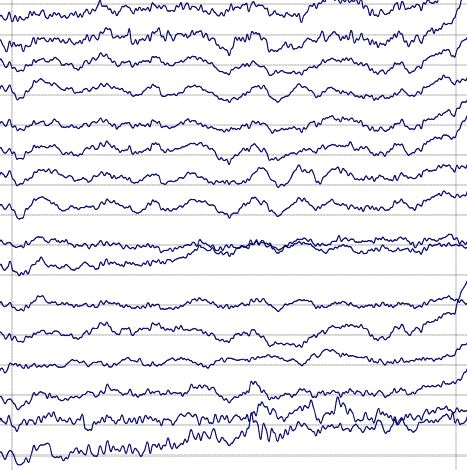
\includegraphics[width=18cm,height=6cm]{eeg.jpg}};

\pic[shift={(3,0,0)}] at (input-east) 
    {RightBandedBox={
        name=conv1,
        caption=conv1,
        xlabel=6,
        ylabel=28,
        zlabel=82,
        fill=\ConvColor,
        bandfill=\ConvReluColor,
        height=28,
        width=6,
        depth=82
        }
    };

\draw [connection]  (input-east)    -- node {\midarrow} (conv1-west);

\pic[shift={ (0,0,0) }] at (conv1-east) 
    {Box={
        name=pool1,
        caption=MaxPool,
        xlabel=6,
        ylabel=14,
        zlabel=40,    
        fill=\PoolColor,
        opacity=0.5,
        height=14,
        width=6,
        depth=40
        }
    };

\pic[shift={(3,0,0)}] at (pool1-east) 
    {RightBandedBox={
        name=conv2,
        caption=conv2,
        xlabel=8,
        ylabel=10,
        zlabel=26,
        fill=\ConvColor,
        bandfill=\ConvReluColor,
        height=10,
        width=8,
        depth=26
        }
    };

\draw [connection]  (pool1-east)    -- node {\midarrow} (conv2-west);

\pic[shift={ (0,0,0) }] at (conv2-east) 
    {Box={
        name=pool2,
        caption=MaxPool,
        xlabel=8,
        ylabel=5,
        zlabel=12,    
        fill=\PoolColor,
        opacity=0.5,
        height=5,
        width=8,
        depth=12
        }
    };

\pic[shift={(2,0,0)}] at (pool2-east) 
    {RightBandedBox={
        name=conv3,
        caption=conv3,
        xlabel=8,
        ylabel=5,
        zlabel=12,
        fill=\ConvColor,
        bandfill=\ConvReluColor,
        height=5,
        width=8,
        depth=12
        }
    };

\draw [connection]  (pool2-east)    -- node {\midarrow} (conv3-west);

\pic[shift={ (0,0,0) }] at (conv3-east) 
    {Box={
        name=pool34,
        caption=MaxPool,
        xlabel=8,
        ylabel=2,
        zlabel=4,    
        fill=\PoolColor,
        opacity=0.5,
        height=2,
        width=8,
        depth=4
        }
    };

\pic[shift={(12,7,0)}] at (pool32-east) 
    {Ball={
        name=sum,
        fill=\SumColor,
        opacity=0.6,
        radius=2.5,
        logo=$+$
        }
    };

\draw [connection]  (pool31-east)    -- node {\midarrow} (sum-west);

\draw [connection]  (pool32-east)    -- node {\midarrow} (sum-west);

\draw [connection]  (pool33-east)    -- node {\midarrow} (sum-west);

\draw [connection]  (pool34-east)    -- node {\midarrow} (sum-west);

\pic[shift={ (5,0,0) }] at (sum-east) 
    {Box={
        name=cascade,
        caption=cascade,
        xlabel=1,
        ylabel=1,
        zlabel=256,
        fill=\FcColor,
        height=3.5,
        width=3.5,
        depth=256
        }
    };

\draw [connection]  (sum-east)    -- node {\midarrow} (cascade-west);

\pic[shift={ (3,0,0) }] at (cascade-east) 
    {RightBandedBox={
        name=fc1,
        caption=fc1,
        xlabel=1,
        ylabel=1,
        zlabel=32,
        fill=\FcFineColor,
        bandfill=\FcReluFineColor,
        height=2.5,
        width=2.5,
        depth=32
        }
    };

\draw [connection]  (cascade-east)    -- node {\midarrow} (fc1-west);

\pic[shift={(3,0,0)}] at (fc1-east) 
    {Box={
        name=softMax,
        caption=SoftMax,
        xlabel=1,
        ylabel=1,
        zlabel=4,
        fill=\SoftmaxColor,
        opacity=0.5,
        height=1,
        width=1,
        depth=4
        }
    };

\draw [connection]  (fc1-east)    -- node {\midarrow} (softMax-west);

\end{tikzpicture}
\end{document}
